\documentclass[14pt]{extbook}
\usepackage{multicol, enumerate, enumitem, hyperref, color, soul, setspace, parskip, fancyhdr} %General Packages
\usepackage{amssymb, amsthm, amsmath, bbm, latexsym, units, mathtools} %Math Packages
\everymath{\displaystyle} %All math in Display Style
% Packages with additional options
\usepackage[headsep=0.5cm,headheight=12pt, left=1 in,right= 1 in,top= 1 in,bottom= 1 in]{geometry}
\usepackage[usenames,dvipsnames]{xcolor}
\usepackage{dashrule}  % Package to use the command below to create lines between items
\newcommand{\litem}[1]{\item#1\hspace*{-1cm}\rule{\textwidth}{0.4pt}}
\pagestyle{fancy}
\lhead{Progress Quiz 4}
\chead{}
\rhead{Version A}
\lfoot{8448-1521}
\cfoot{}
\rfoot{Fall 2020}
\begin{document}

\begin{enumerate}
\litem{
Solve the linear equation below. Then, choose the interval that contains the solution.\[ \frac{-3x + 4}{7} - \frac{6x + 5}{8} = \frac{-3x + 3}{5} \]\begin{enumerate}[label=\Alph*.]
\item \( x \in [-7.65, -5.62] \)
\item \( x \in [-1.45, -0.58] \)
\item \( x \in [0.99, 1.44] \)
\item \( x \in [-0.6, 0.37] \)
\item \( \text{There are no real solutions.} \)

\end{enumerate} }
\litem{
First, find the equation of the line containing the two points below. Then, write the equation as $ y=mx+b $ and choose the intervals that contain $m$ and $b$.\[ (-6, 11) \text{ and } (3, 4) \]\begin{enumerate}[label=\Alph*.]
\item \( m \in [-2.1, -0.7] \hspace*{3mm} b \in [6.03, 8.21] \)
\item \( m \in [-2.1, -0.7] \hspace*{3mm} b \in [0.92, 1.05] \)
\item \( m \in [-0.2, 1.1] \hspace*{3mm} b \in [1.47, 2.37] \)
\item \( m \in [-2.1, -0.7] \hspace*{3mm} b \in [-6.81, -5.38] \)
\item \( m \in [-2.1, -0.7] \hspace*{3mm} b \in [15.92, 17.76] \)

\end{enumerate} }
\litem{
Write the equation of the line in the graph below in Standard form $Ax+By=C$. Then, choose the intervals that contain $A, B, \text{ and } C$.
\begin{center}
    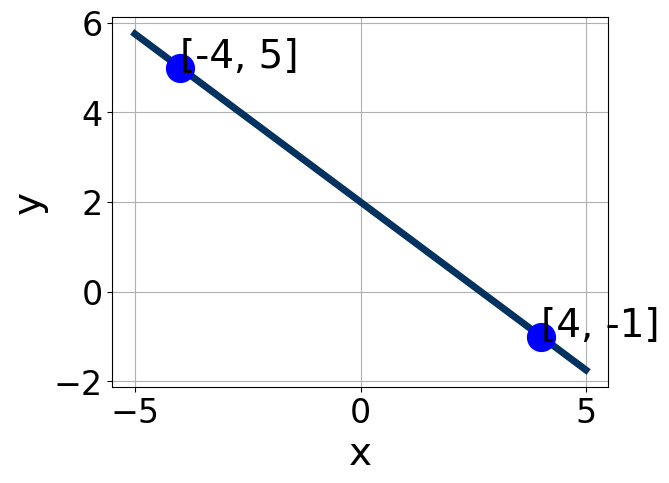
\includegraphics[width=0.5\textwidth]{../Figures/linearGraphToStandardCopyA.png}
\end{center}
\begin{enumerate}[label=\Alph*.]
\item \( A \in [-2.2, 1.1], \hspace{3mm} B \in [-2.9, 0], \text{ and } \hspace{3mm} C \in [-2, 0] \)
\item \( A \in [-2.2, 1.1], \hspace{3mm} B \in [0, 2.3], \text{ and } \hspace{3mm} C \in [1, 7] \)
\item \( A \in [0.9, 4.4], \hspace{3mm} B \in [3.5, 6.5], \text{ and } \hspace{3mm} C \in [9, 11] \)
\item \( A \in [0.9, 4.4], \hspace{3mm} B \in [-5.6, -4.1], \text{ and } \hspace{3mm} C \in [-18, -3] \)
\item \( A \in [-3.5, -2.3], \hspace{3mm} B \in [3.5, 6.5], \text{ and } \hspace{3mm} C \in [9, 11] \)

\end{enumerate} }
\litem{
Solve the linear equation below. Then, choose the interval that contains the solution.\[ \frac{-5x + 9}{4} - \frac{-3x -8}{2} = \frac{-4x -9}{3} \]\begin{enumerate}[label=\Alph*.]
\item \( x \in [-17.42, -15.42] \)
\item \( x \in [-0.79, 1.21] \)
\item \( x \in [-6.84, -4.84] \)
\item \( x \in [-5.62, -1.62] \)
\item \( \text{There are no real solutions.} \)

\end{enumerate} }
\litem{
Find the equation of the line described below. Write the linear equation as $ y=mx+b $ and choose the intervals that contain $m$ and $b$.\[ \text{Perpendicular to } 7 x - 5 y = 14 \text{ and passing through the point } (-3, 7). \]\begin{enumerate}[label=\Alph*.]
\item \( m \in [-1.11, -0.15] \hspace*{3mm} b \in [-5.16, -4.77] \)
\item \( m \in [-1.11, -0.15] \hspace*{3mm} b \in [3.36, 5.13] \)
\item \( m \in [-1.11, -0.15] \hspace*{3mm} b \in [9.81, 10.68] \)
\item \( m \in [0.29, 1.74] \hspace*{3mm} b \in [8.53, 9.62] \)
\item \( m \in [-1.89, -0.76] \hspace*{3mm} b \in [3.36, 5.13] \)

\end{enumerate} }
\litem{
Find the equation of the line described below. Write the linear equation as $ y=mx+b $ and choose the intervals that contain $m$ and $b$.\[ \text{Parallel to } 6 x - 5 y = 3 \text{ and passing through the point } (3, -7). \]\begin{enumerate}[label=\Alph*.]
\item \( m \in [1.16, 1.39] \hspace*{3mm} b \in [-10.82, -10.35] \)
\item \( m \in [1.16, 1.39] \hspace*{3mm} b \in [10.01, 10.65] \)
\item \( m \in [0.02, 1.15] \hspace*{3mm} b \in [-10.82, -10.35] \)
\item \( m \in [-1.93, -0.58] \hspace*{3mm} b \in [-4.02, -3.1] \)
\item \( m \in [1.16, 1.39] \hspace*{3mm} b \in [-10.01, -9.77] \)

\end{enumerate} }
\litem{
First, find the equation of the line containing the two points below. Then, write the equation as $ y=mx+b $ and choose the intervals that contain $m$ and $b$.\[ (-8, 7) \text{ and } (4, 11) \]\begin{enumerate}[label=\Alph*.]
\item \( m \in [-0.13, 0.51] \hspace*{3mm} b \in [5.49, 8.68] \)
\item \( m \in [-1.46, 0.05] \hspace*{3mm} b \in [11.91, 13.47] \)
\item \( m \in [-0.13, 0.51] \hspace*{3mm} b \in [-10.73, -9.01] \)
\item \( m \in [-0.13, 0.51] \hspace*{3mm} b \in [13.63, 16.14] \)
\item \( m \in [-0.13, 0.51] \hspace*{3mm} b \in [9.28, 10.04] \)

\end{enumerate} }
\litem{
Solve the equation below. Then, choose the interval that contains the solution.\[ -4(-13x -11) = -12(-2x + 7) \]\begin{enumerate}[label=\Alph*.]
\item \( x \in [1.12, 1.46] \)
\item \( x \in [-2.51, -1.33] \)
\item \( x \in [-5.82, -4.35] \)
\item \( x \in [-0.04, 1.19] \)
\item \( \text{There are no real solutions.} \)

\end{enumerate} }
\litem{
Solve the equation below. Then, choose the interval that contains the solution.\[ -17(-11x -3) = -8(-7x + 2) \]\begin{enumerate}[label=\Alph*.]
\item \( x \in [-0.02, 0.36] \)
\item \( x \in [-0.21, 0.09] \)
\item \( x \in [-0.57, -0.5] \)
\item \( x \in [-0.28, -0.22] \)
\item \( \text{There are no real solutions.} \)

\end{enumerate} }
\litem{
Write the equation of the line in the graph below in Standard form $Ax+By=C$. Then, choose the intervals that contain $A, B, \text{ and } C$.
\begin{center}
    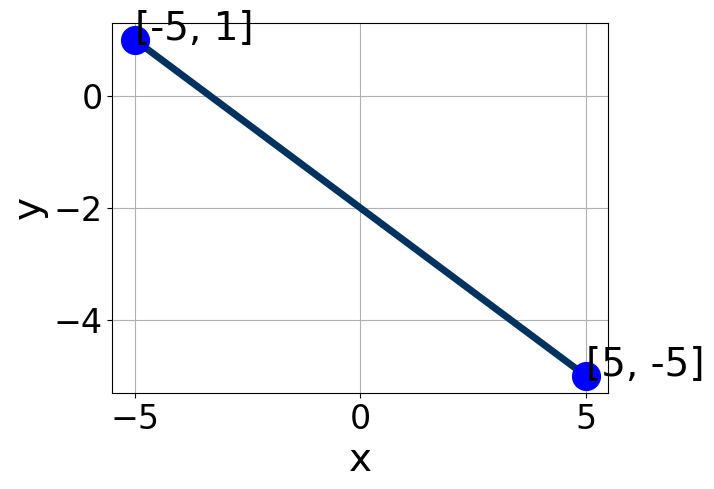
\includegraphics[width=0.5\textwidth]{../Figures/linearGraphToStandardA.png}
\end{center}
\begin{enumerate}[label=\Alph*.]
\item \( A \in [4, 9], \hspace{3mm} B \in [3.6, 5.5], \text{ and } \hspace{3mm} C \in [-21, -17] \)
\item \( A \in [-6, -2], \hspace{3mm} B \in [-9, -2], \text{ and } \hspace{3mm} C \in [17, 24] \)
\item \( A \in [4, 9], \hspace{3mm} B \in [-9, -2], \text{ and } \hspace{3mm} C \in [17, 24] \)
\item \( A \in [-2.2, 3.8], \hspace{3mm} B \in [-0.5, 3.3], \text{ and } \hspace{3mm} C \in [-8, -2] \)
\item \( A \in [-2.2, 3.8], \hspace{3mm} B \in [-3.3, 0.8], \text{ and } \hspace{3mm} C \in [2, 5] \)

\end{enumerate} }
\end{enumerate}

\end{document}